\documentclass{beamer}
% \documentclass[handout]{beamer}

\usetheme{Madrid}
\usepackage[style=gb7714-2015]{biblatex}
\addbibresource{ref.bib}
\usepackage{amsmath, amsthm, amssymb}
\usepackage{algorithm2e}
\usepackage{graphicx}
\graphicspath{{image/}}
\DeclareGraphicsExtensions{.png,PNG,.jpg,.JPG,.jpeg,.JPEG,.pdf,.PDF}

\title{Double Auction on Social Network}
\author{Peng Cheng, Huizhe Su, Jingtian Hu, Weiming Luo, Liyu Yang}
\date{\today}

\AtBeginSection[] % Do nothing for \section*
{
	\begin{frame}<beamer>
		\frametitle{Outline}
		\tableofcontents[currentsection]
	\end{frame}
}

\begin{document}

\frame{\titlepage}
\begin{frame}{Contents}
	\tableofcontents
\end{frame}

\section{Introduction}

\subsection{Background}

\begin{frame}{Mechanism Design on Social Network}
	\begin{center}
		
\includegraphics[width=0.4\textwidth]{social-networks-icons}
		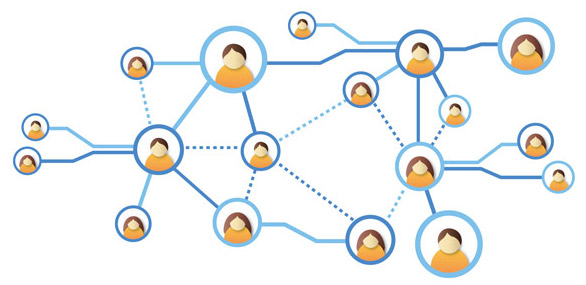
\includegraphics[width=0.4\textwidth]{social-network-graph}
	\end{center}

	\begin{block}{implication of the connectivity of social networks}
		\begin{description}
			\item[opportunity] social level welfare expansion and boost in individual utility
			\item[challenge] possibility of manipulation in diffusion and bidding
		\end{description}
	\end{block}
\end{frame}
\begin{frame}{Double Auction}
	\begin{columns}
		\begin{column}{0.2\textwidth}
			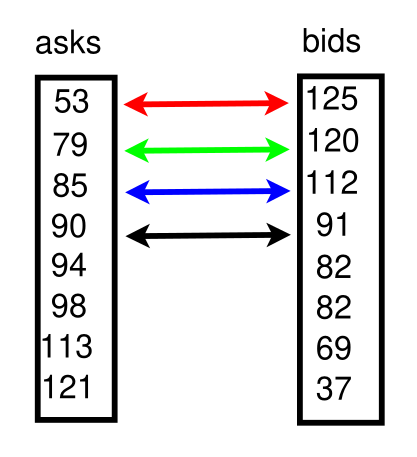
\includegraphics[height=0.3\textheight]{double-auction-example}
		\end{column}
		\begin{column}{0.8\textwidth}
			\begin{block}{Participants}
				\begin{itemize}
					\item two groups of disjoint players, buyers and sellers.
					\item each buyer $b_i$ is willing to sell an item at price higher than $v^b_i$
					\item each seller $s_j$ aims to sell an item at price lower than $v^s_j$
				\end{itemize}
			\end{block}
			\begin{block}{Mechanism}
				\begin{description}
					\item[input] reported valuation from buyers and sellers $(\hat v^b, \hat v^s)$
					\item[output] allocation $(\pi^b,\pi^s)$ and payment $(p^b,p^s)$, determining the trade pairs and prices
				\end{description}
			\end{block}
		\end{column}
	\end{columns}

\end{frame}
\begin{frame}{Bilateral Trades on a Social Network}
	\begin{columns}
		\begin{column}{0.4\textwidth}
			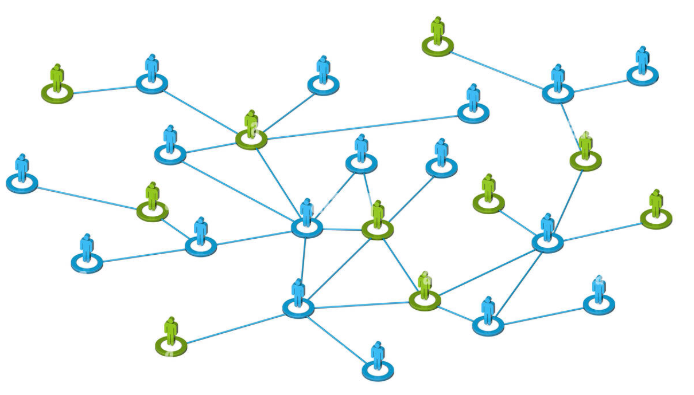
\includegraphics[height=0.3\textheight]{exchange-trade-social-network}
		\end{column}
		\begin{column}{0.5\textwidth}
			\begin{block}{New Restrictions}
				\begin{itemize}
					\item Trade only happens on neighbouring players
					\item Only a small proportion of the social network is aware of the trade.
				\end{itemize}
			\end{block}
		\end{column}
	\end{columns}

	\begin{alertblock}{Complicated Strategies}
		\begin{description}
			\item[diffuse] Inviting neighbours for potential rewards
			\item[block] Blocking competitors from entering the auction
		\end{description}
	\end{alertblock}
\end{frame}

\subsection{Prior Work}
\begin{frame}{Existing Social Network Auction Mechanisms}
	\begin{center}
		\begin{tabular}{ll|l|l}
			players   & supply         & restriction           & mechanism \\
			\hline
			one-sided & single item    & arbitrary network     & IDM       \\
			one-sided & multiple items & arbitrary network     & MUDAN     \\
			two-sided & single item    & disjoint buyer groups & DNA       \\
		\end{tabular}
	\end{center}
\end{frame}

\begin{frame}{IDM: one sided, single item}
	\begin{columns}
		\begin{column}{0.3\textwidth}
			\begin{center}
				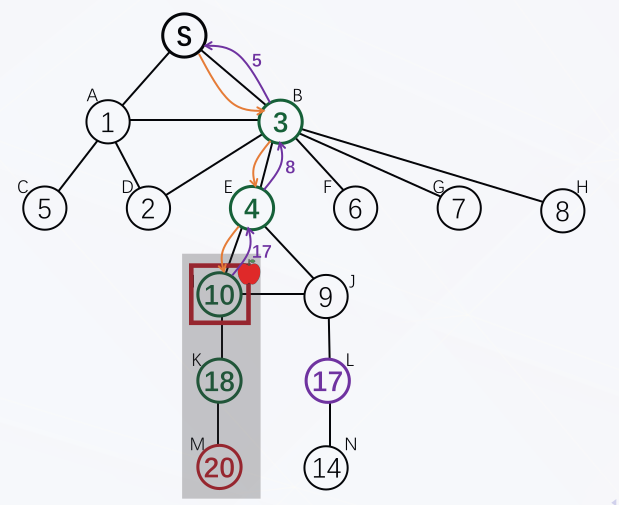
\includegraphics[width=\textwidth]{IDM-example}
			\end{center}
		\end{column}
		\begin{column}{0.7\textwidth}
			\begin{block}{Brief of IDM}
				\begin{enumerate}
					\item Determine the critical path to agent with highest valuation
					\item Payment: Outside subtree highest price
					\item Resaling if possible
				\end{enumerate}
			\end{block}
			\begin{block}{Properties}
				IC, IR, WBB; Efficiency better than local auction
			\end{block}
		\end{column}
	\end{columns}
\end{frame}
\begin{frame}{MUDAN: one sided, multiple items}
	\begin{columns}
		\begin{column}{0.3\textwidth}
			\begin{center}
				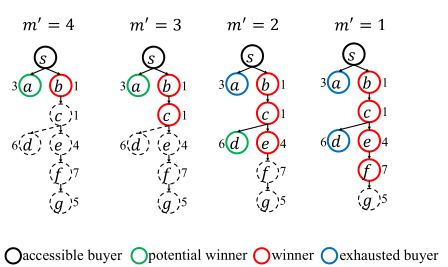
\includegraphics[width=\textwidth]{MUDAN-example}
			\end{center}
		\end{column}
		\begin{column}{0.7\textwidth}
			\begin{block}{Brief of MUDAN}
				\begin{enumerate}
					\item The priority of a buyer is the number of neighbours invited by him.
					\item Iterative exploration of the network based on the priority.
					\item Sell an item to the player with highest priority.\\
					      Price is the $m'+1$-th highest\footnote{$m'$ is the number of remained items to sell}.
				\end{enumerate}
			\end{block}
			\begin{block}{Properties}
				IC, IR, WBB, $1/m$-efficiency
			\end{block}
		\end{column}
	\end{columns}
\end{frame}
\begin{frame}{DNA: two sided, single item per seller}
	\begin{columns}
		\begin{column}{0.3\textwidth}
			\begin{center}
				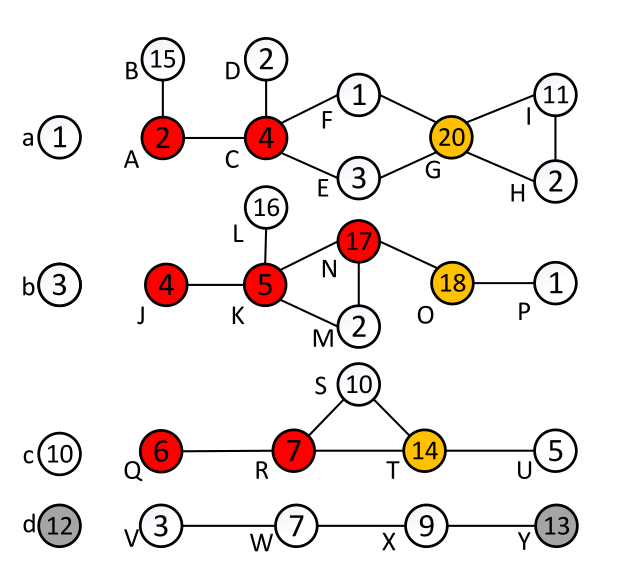
\includegraphics[width=\textwidth]{DNA-example}
			\end{center}
		\end{column}
		\begin{column}{0.7\textwidth}
			\begin{block}{Brief of DNA}
				\begin{enumerate}
					\item Partition graph into buyer groups
					\item Sort buyer groups by the highest price within groups.
					\item McAfee's mechanism determine the allocation and payment for sellers.
					\item Sell items to the buyer with highest bid in each group.
					\item VCG-alike payment/reward for buyers.
				\end{enumerate}
			\end{block}
			\begin{block}{Properties}
				IC, IR, WBB
			\end{block}
		\end{column}
	\end{columns}
\end{frame}

\begin{frame}{Limitation of Existing Mechanisms}
	\begin{center}
		\begin{tabular}{ll|l|l}
			players   & supply         & restriction             & mechanism \\
			\hline
			one-sided & single item    & arbitrary network       & IDM       \\
			one-sided & multiple items & arbitrary network       & MUDAN     \\
			two-sided & single item    & disjoint buyer groups   & DNA       \\
			two-sided & single item    & connected buyers groups & (unknown) \\
		\end{tabular}
	\end{center}

	\begin{block}{Our Goal}
		Design an double auction mechanism applicable to realistic social networks
	\end{block}
\end{frame}



\section{Problem Setting}
\subsection{Model of Double Auction on Social Network}
\begin{frame}{Model of Double Auction on Social Network}
	\begin{block}{Components of the double auction}
		\begin{description}
			\item[players] Buyers $B$ and Sellers $S$, which are disjoint $B\cap S=\varnothing$.
			\item[valuation] Afforable price of buyers $v^b_i$ and reserved price of sellers $v^s_j$
			\item[social network]
				Each seller $s_i\in S$ can only interact with $N_s(s_i) \subseteq S$.\\
				Each buyer $b_j\in B$ can only interact with $N_b(b_j) \subseteq B$.
			\item[initial/heads] $S_0\subseteq S$, every $s_i\in S_0$ knows $NB(s_i) \subseteq B$.\\
				$B_0\subseteq B$, every $b_j\in B_0$ knows $NS(b_j) \subseteq S$.
			\item[utility] $u^b_i$ for buyer and $u^s_i$ for sellers, where
		\end{description}
		\[
			u^b_i = \begin{cases}
				v^b_i - p^b_i & \text{buy at price $p^b_i$} \\
				0             & \text{otherwise}
			\end{cases}
			\quad
			u^s_i = \begin{cases}
				p^s_i - v^s_i & \text{sold at price $p^s_i$} \\
				0             & \text{otherwise}
			\end{cases}
		\]
	\end{block}
\end{frame}
\subsection{Diffusion Double Auction Mechanism}
\begin{frame}{Model of Diffusion Double Auction Mechanism}
	\begin{block}{Strategies of agents}
		\begin{description}
			\item[diffusion action] Every agent $a\in S\cup B$ invite $\hat N(a) \subseteq N(a)$ into the market.
			\item[bid action] Buyers and sellers report valuation $\hat v^b, \hat v^s$
		\end{description}
	\end{block}

	\begin{block}{Execution of the Mechanism}
		\begin{description}
			\item[Payment] Determine the price and rewards.
				$p^s_i: S\to \mathbb{R}, p^s_j: B\to \mathbb{R}$.
			\item[Allocation] Determine the trade pairs.
				$\pi^s_i: S\to \{0,1\}, \pi^s_j: B\to \{0,1\}$.
			\item[Execution] Computing feasible trades.
		\end{description}
	\end{block}
\end{frame}

\subsection{Expected Property}
\begin{frame}{Goals}
	\begin{block}{Desirable Properties of a Double Auction Mechanism}
		\begin{description}
			\item[Incentive Compatbility] Or truthfulness.
			\item[Indivdual Rationality] Or participation.
			\item[Weakly Budget Balance] Or non-deficit.
			\item[Economics Efficient] Or social welfare maximizing
		\end{description}
	\end{block}

	\alert{these properties may not be achieved in by one mechanism\footnote{\textit{Efficiency in truthful auctions via a social network}. arXiv:1904.12422}}
\end{frame}


\section{Attempts}
\subsection{IDM with Leave and Share}
\begin{frame}{Attempts 1: Adoption of IDM}
	Insight:
	We want people who have higher valuation hold the item,
	so resale mechanism is preferred.\\\pause
	Initial attempts:
	\begin{enumerate}
		\item Sort the seller in ascending order and the buyer in descending order.
		\item Run IDM.
		\item If the payment is higher than the first seller's expectation, the seller is matched.
		      Otherwise, stop.
		\item The winner leave the network and share its connection.
		\item Go to 2.
	\end{enumerate}
\end{frame}
\begin{frame}{Seller not IC: Counterexample}
	\begin{center}
		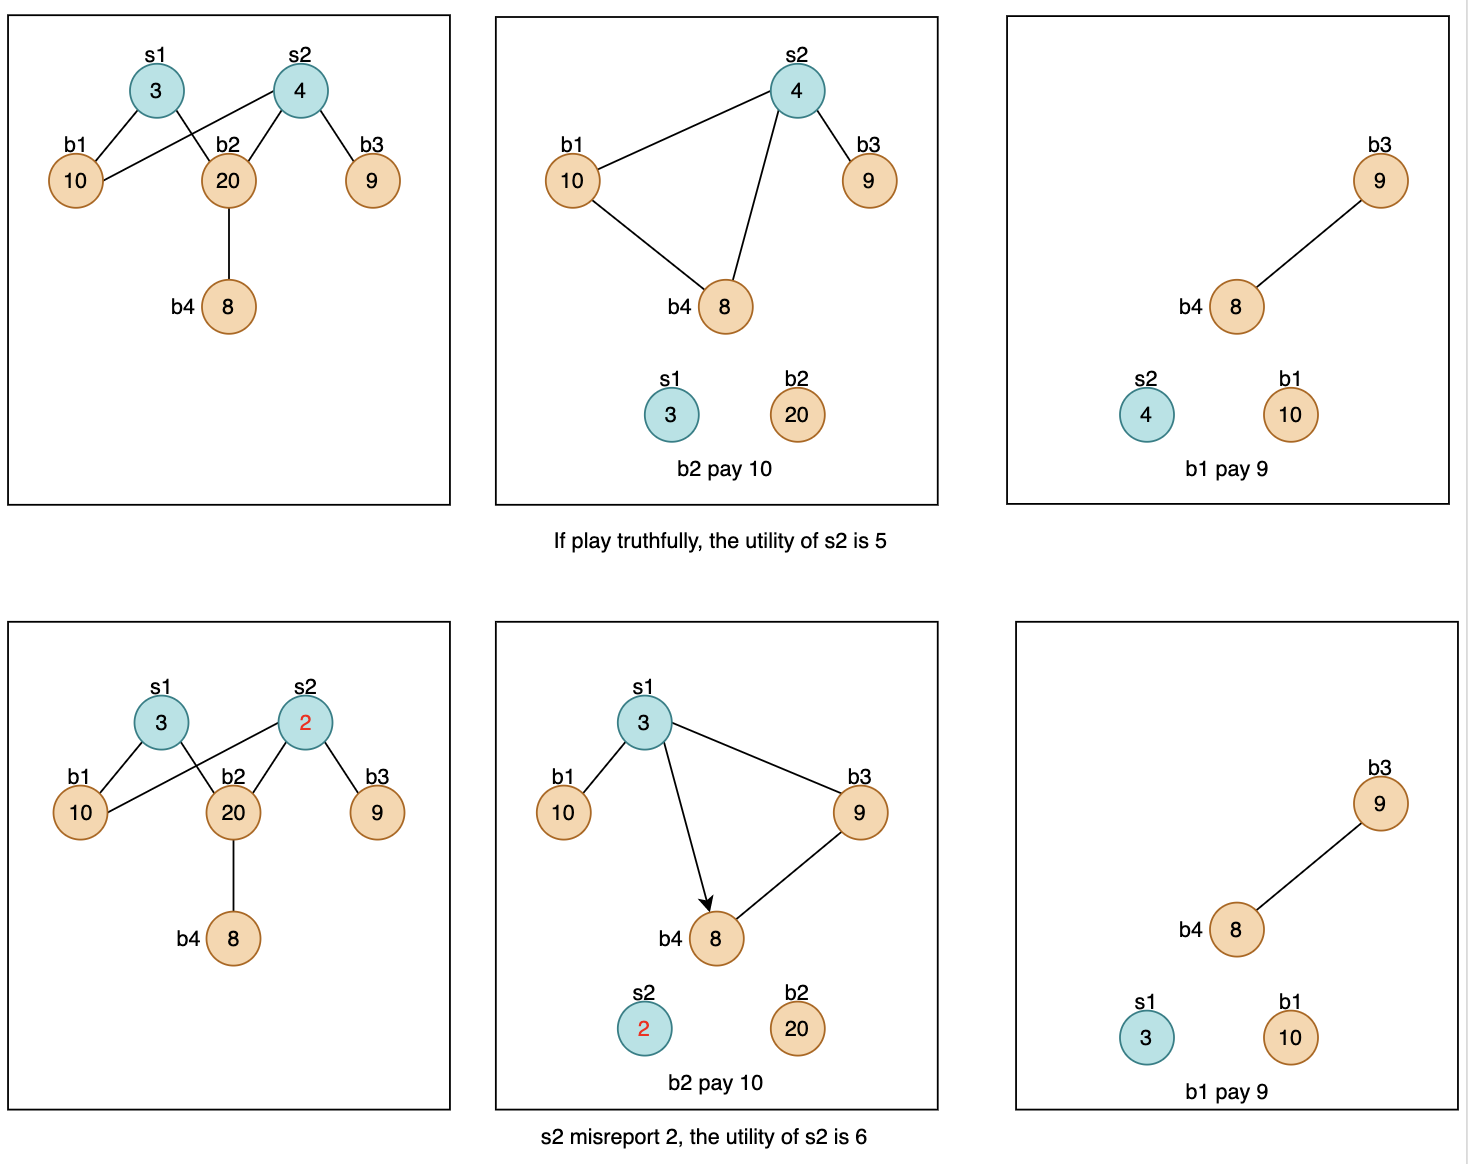
\includegraphics[width=0.85\textwidth]{IDMCounter1}
	\end{center}
\end{frame}
\begin{frame}{Fix of the mechanism}
	\begin{enumerate}
		\item Sort the seller in ascending order and the buyer in descending order.
		\item \textcolor{red}{Let \(m = \) the number of the remaining seller}
		\item Run IDM. When calculating the payment, omit the \textcolor{red}{first \(m\) higher bids}.
		\item If the payment is higher than the first seller's expectation, the seller is matched.
		      Otherwise, stop.
		\item The winner leave the network and share its connection.
		\item Go to 2.
	\end{enumerate}
	Now sellers will play truthfully...\\\pause
	However, the buyer have a chance to misreport.
\end{frame}
\begin{frame}{Extra reward from resale}
	\begin{center}
		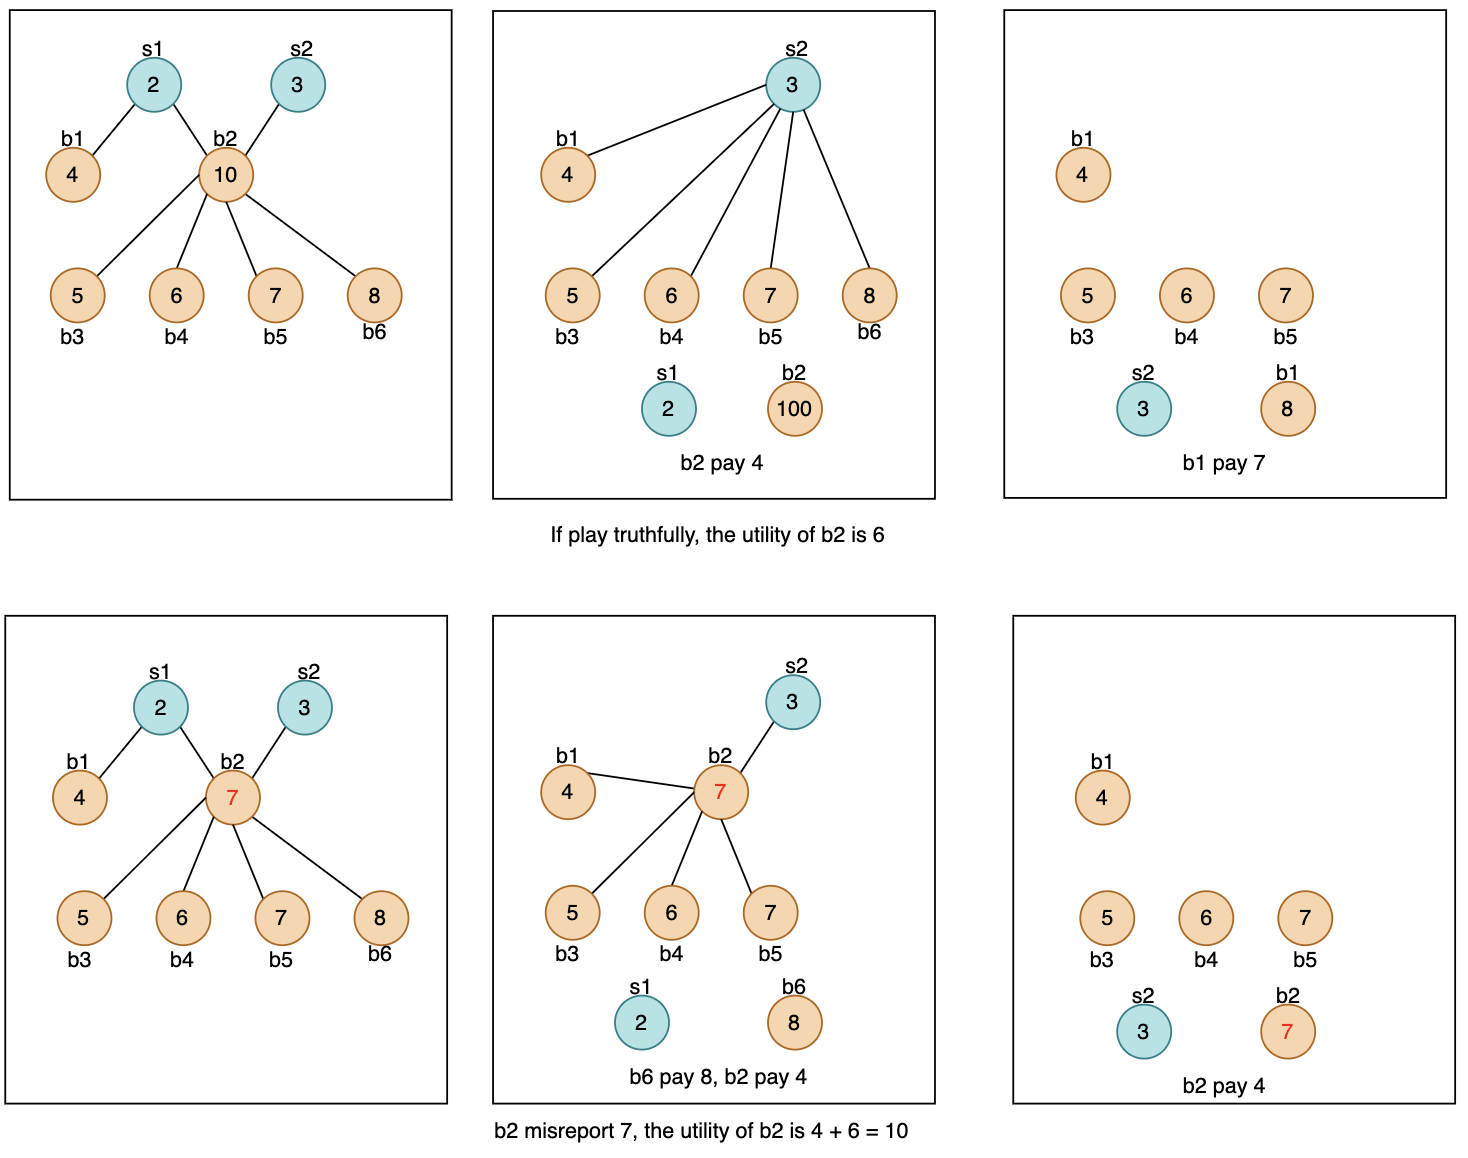
\includegraphics[width=0.8\textwidth]{IDMCounter2}
	\end{center}
\end{frame}
\begin{frame}{Extra reward from resale}
	\begin{center}
		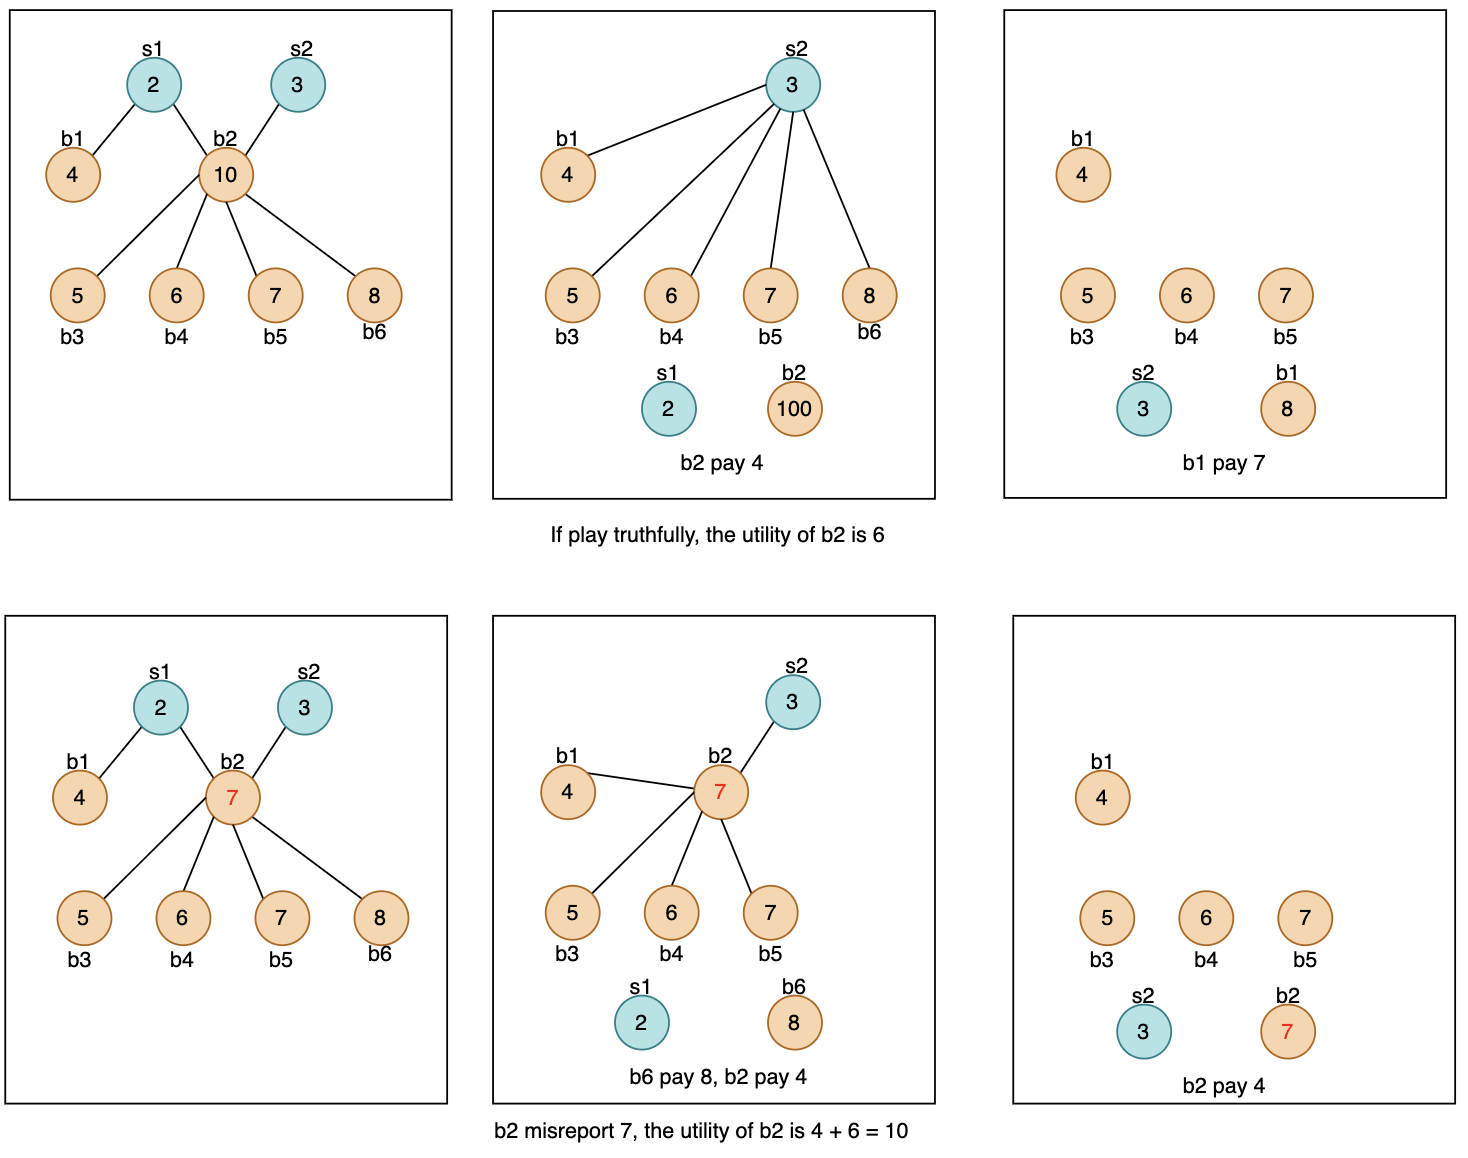
\includegraphics[width=0.6\textwidth]{IDMCounter2}
	\end{center}
	This problem come with any resale mechanism that rewards player who plays as a reseller.
	Therefore, we have to abandon this kind of mechanism.

\end{frame}
\subsection{DNA with Graph Partition}
\begin{frame}{Attempts 2: Connected buyer group}
	\begin{itemize}
		\item Recall that: DNA runs on several isolated buyer groups with one head buyers in each group connected with seller.
		\item Intuition: If the graph has the property that the buyer conncets to at most one seller, the the buyer can be viewed as head buyer.
		\item If we have a method to partition the graph into different buyer group, we can then run DNA on that graph.
	\end{itemize}
\end{frame}
\begin{frame}{Graph Partition}
	Partition Algorithm:
	\begin{enumerate}
		\item Calculate each buyer's depth by finding the minimal distance to the nearest head buyer.
		\item Remove the edge between nodes with the same level.
		\item Let each head buyer be a buyer group and keep recording each buyer group's highest valuation.
		\item Start from the deepest layer and the node with highest valuation.
		\item Find critical paths to all the buyer groups where the node has the highest value among all the nodes on the path.
		\item Omit the nodes have no critical path.
		\item If there's only one critical path, add all the nodes on that path to the corresponding buyer group.
		\item Otherwise, choose the path to the buyer group with lowest highest valuation.
		\item  Repeat untill no new buyers can be added to a group.
		\item Randomly add the omitted buyers.
	\end{enumerate}
\end{frame}
\begin{frame}{Example}
	\begin{center}
		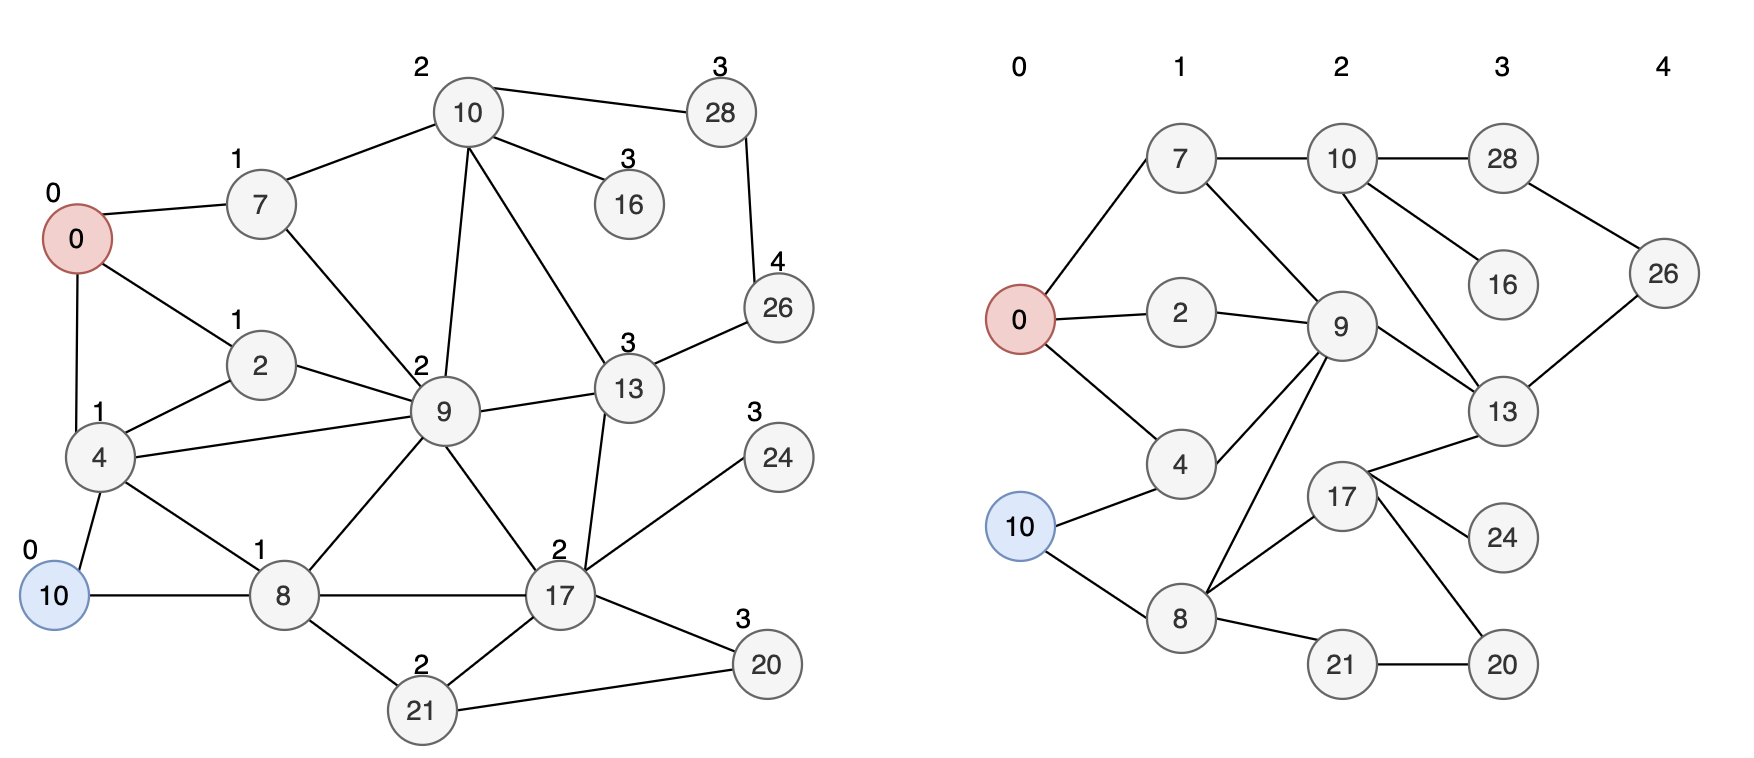
\includegraphics[width=\textwidth]{Graph01}
	\end{center}
\end{frame}
\begin{frame}{Example}
	\begin{center}
		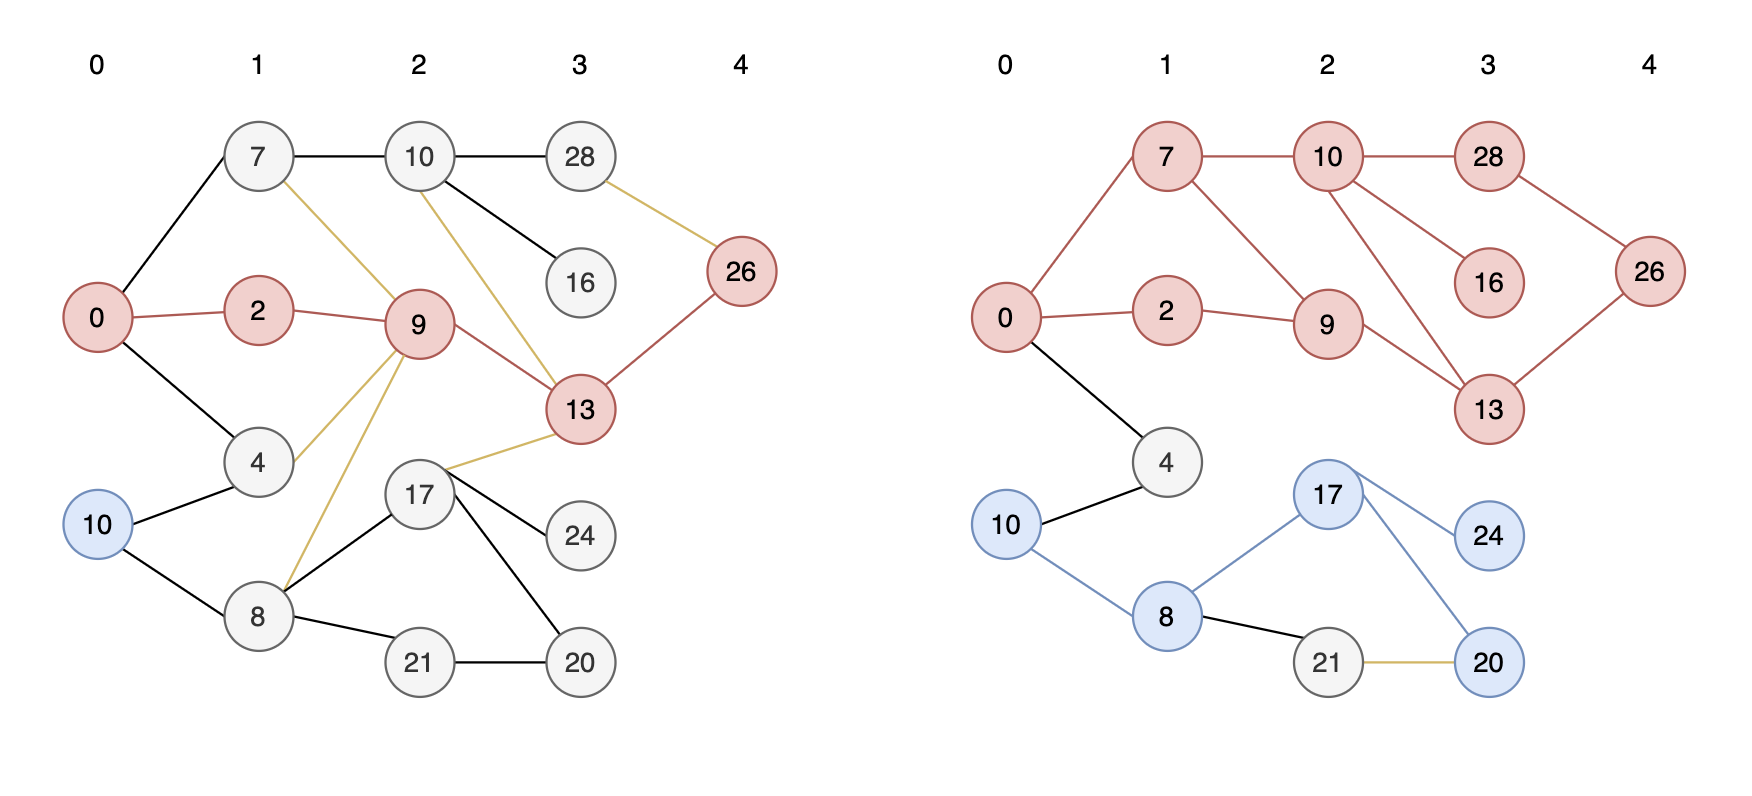
\includegraphics[width=\textwidth]{Graph02}
	\end{center}
\end{frame}
\begin{frame}{Example}
	\begin{center}
		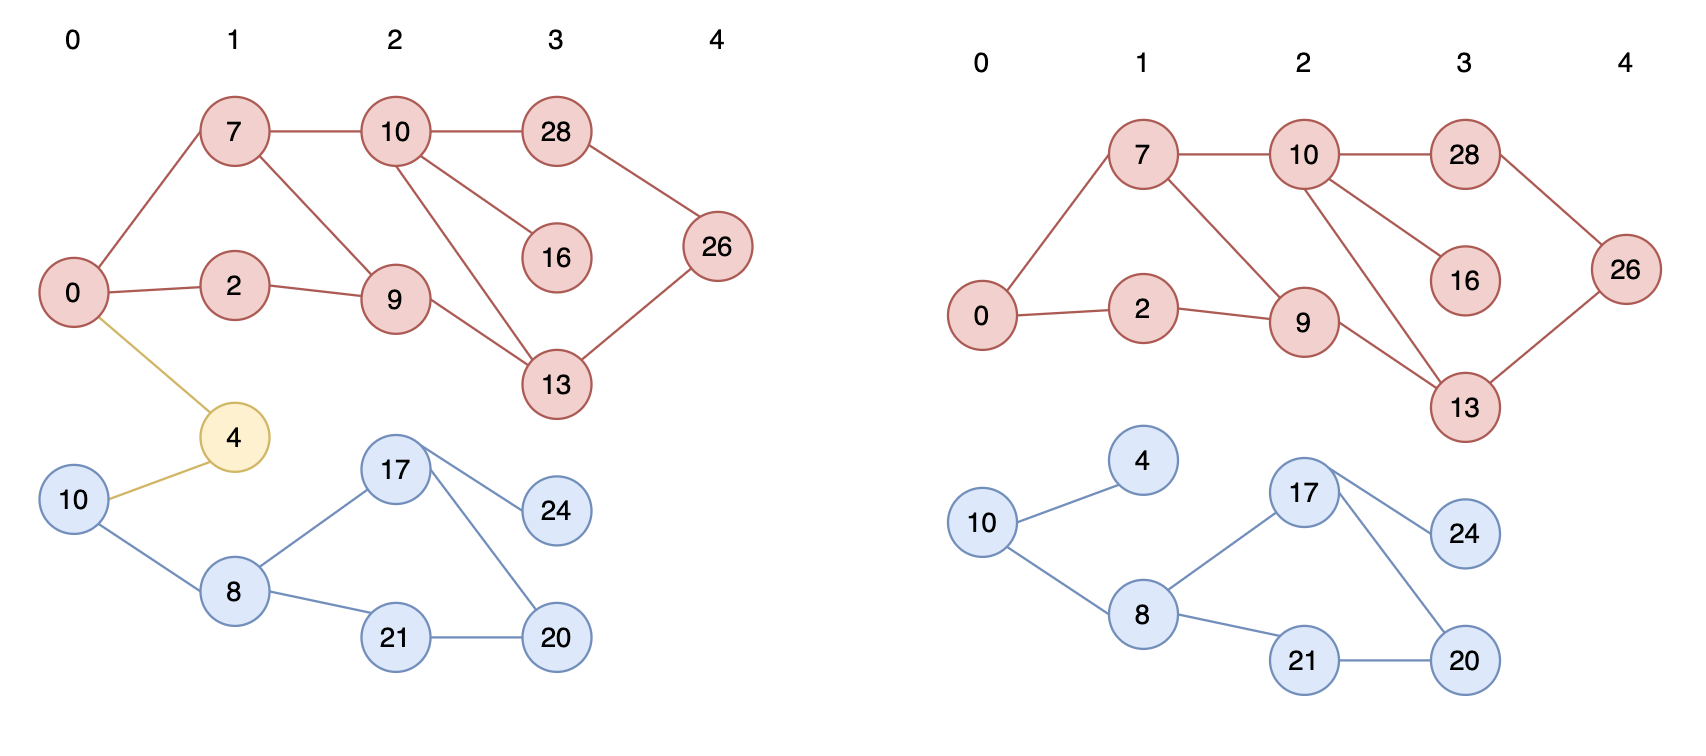
\includegraphics[width=\textwidth]{Graph03}
	\end{center}
\end{frame}
\begin{frame}{Properties}
	However, we are not sure if this mechanism is IC. The proof is beyond our capacity, but we have some vague directions that may be helpful:
	\begin{itemize}
		\item If the buyer misreport more and successfully get the item, his utility will be negative (DNA's IC).
		\item If the buyer misreport less, he will risk the chance to lose the item.
		\item If the buyer misreport less to get into another buyer group, he will enter a group with more competitive buyers. This may decrease his utility.
		\item If the buyer misreport more to get into another group, either he will lose the item or he will get a negative utility.
	\end{itemize}
\end{frame}
\subsection{MUDAN on buyer network}
\begin{frame}{Attempts 3: Reduced seller network}
	There exists some situation that the network cannot be partitioned: When multiple sellers are connected to one buyer.\\\pause
	\begin{itemize}
		\item Insight: This is very similar to multi-unit auction on social network with reserved prices.
		\item Therefore, we can try to adopt the currently IC mechanism on this setting: MUDAN.
		\item Since all the seller are connected together, the sequence of selling is not important.
	\end{itemize}

\end{frame}
\begin{frame}{Club Auction}
	Algorithm:
	\begin{enumerate}
		\item Let \(m = \) the number of sellers. For convenience, suppose that: \(v^s_1 < v^s_2 < \ldots < v^s_m\).
		\item Run MUDAN with \(m\) items.
		\item Let \(p = \) the sum of the buyers' payments given by MUDAN.
		\item If for all \(v^s_i \geq \frac p m\), then let \(p^s = -\frac p m\) be the payment of the seller.
		\item Otherwise, let \(m = m - 1\) and go to 2.
	\end{enumerate}
\end{frame}
\begin{frame}{Example}
	\begin{center}
		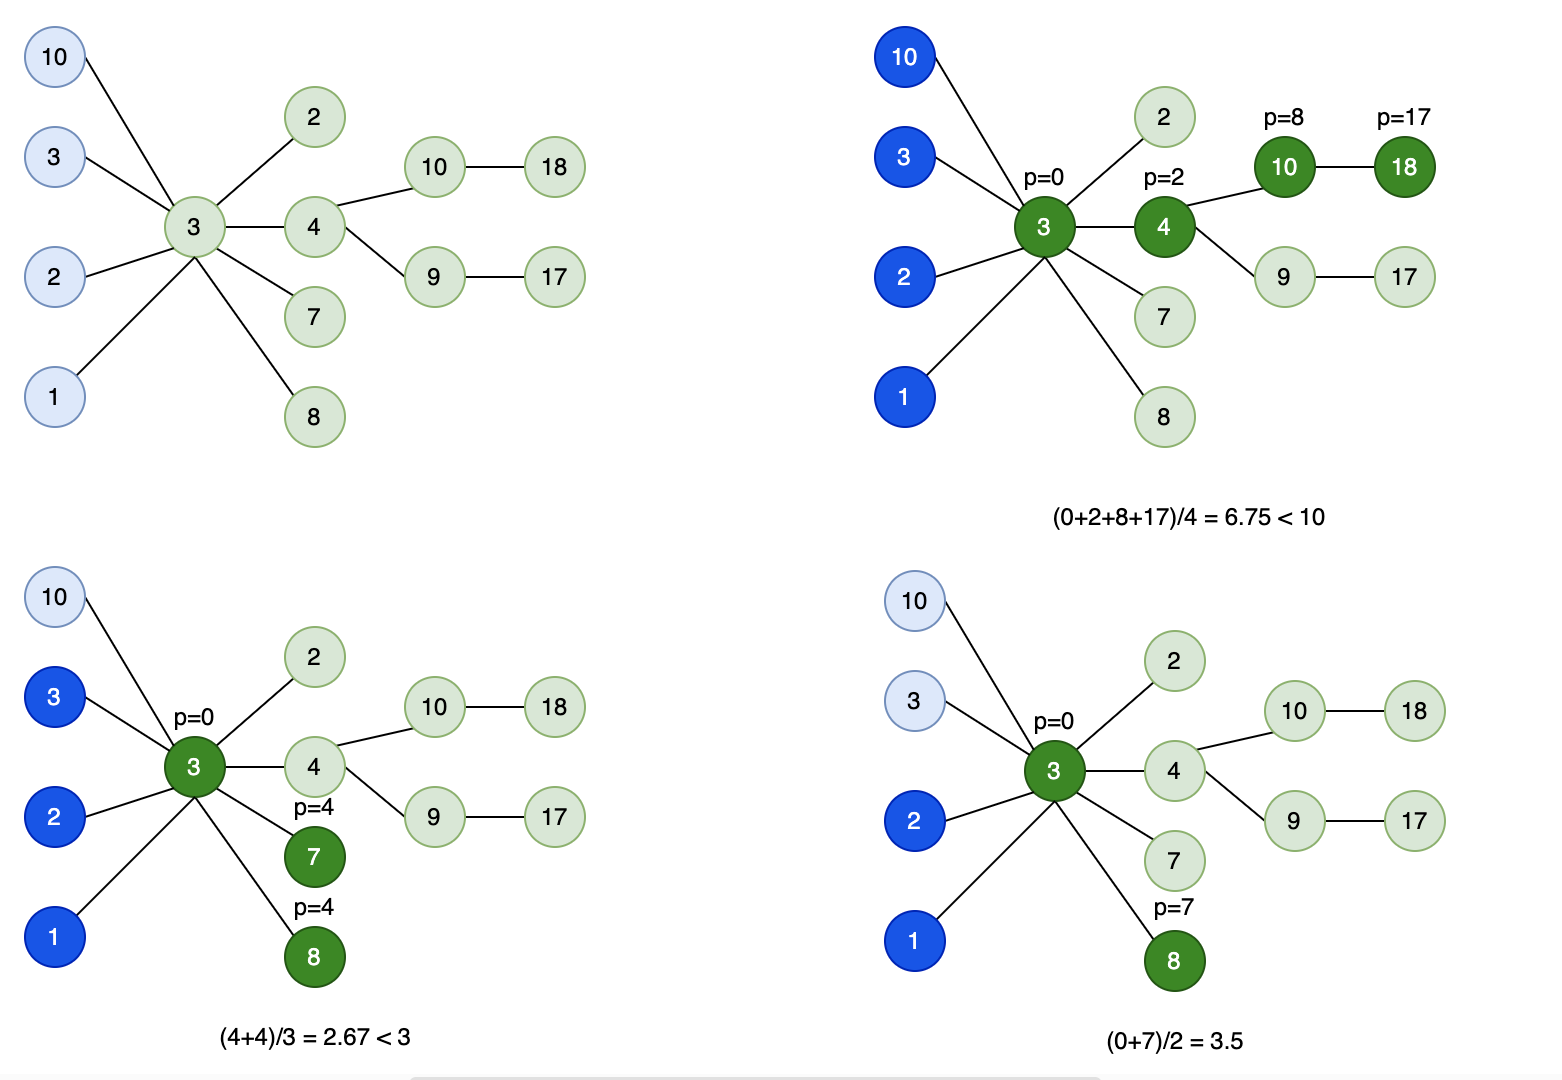
\includegraphics[width=0.9\textwidth]{MUDAN}
	\end{center}
\end{frame}
\begin{frame}{properties}
	The Mechanism is IR, IC and BB.\\ \pause
	IR and BB are trivial.\\
	The sketch of the proof for IC:
	\begin{itemize}
		\item The buyer will play truthfully since MUDAN is IC.
		\item If \(v^s_i < p^s\) and the buyer misreport \(v^{s*}_i > p^s\), his utility will become negative.
		\item If \(v^s_i > p^s\) and the buyer misreport \(v^{s*}_i < p^s\), his utility will decrease to zero.
		\item Under other circumstances, the utility of the buyer will not change.
	\end{itemize}
	\pause
	Any other IC mechanism besides MUDAN also work.
\end{frame}

\section{Summary}
\subsection{Conclusion}
\begin{frame}{Conclusion}
	\begin{itemize}
		\item This problem can be devide into three classes based on the complexity of the graph.
	\end{itemize}
	\begin{columns}
		\begin{column}{0.3\textwidth}
			% Sellers all connected to one buyers.
			\begin{center}
				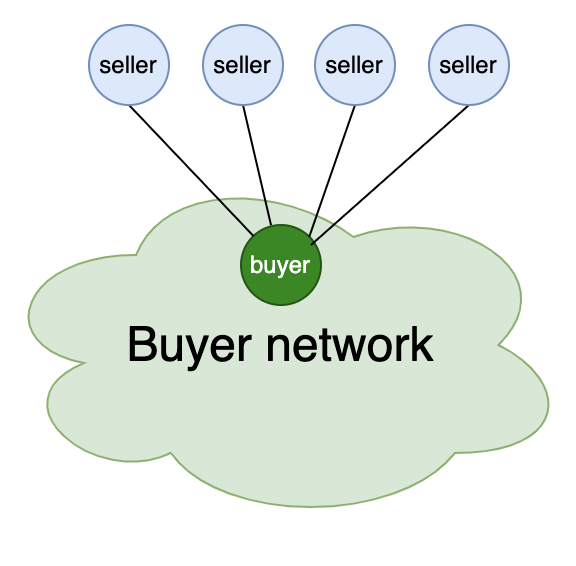
\includegraphics[width=\textwidth]{NetworkStructure1}
			\end{center}
			Club Auction.
		\end{column}
		\begin{column}{0.3\textwidth}
			% Sellers are connected to multiple buyers but have a one-to-one relationship with the head buyers.
			\begin{center}
				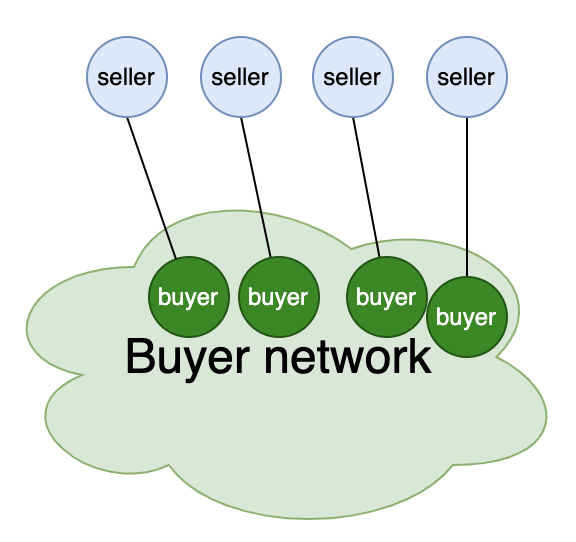
\includegraphics[width=\textwidth]{NetworkStructure3}
			\end{center}
			DNA with graph partition.
		\end{column}
		\begin{column}{0.3\textwidth}
			% Sellers are connected to multiple buyers and head buyers can connect to multiple sellers.
			\begin{center}
				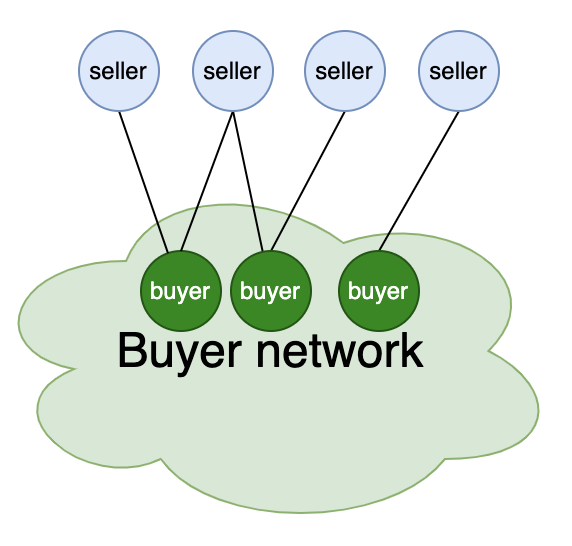
\includegraphics[width=\textwidth]{NetworkStructure2}
			\end{center}
			Combination of the other two networks.
		\end{column}
	\end{columns}
\end{frame}


\subsection{Future Work}
\begin{frame}{Future Work}
	\begin{itemize}

		\item Club Auction depends on multi-unit Single Auction Mechanism.
		      \begin{itemize}
			      \item Find other multi-unit Single Auction Mechanism.
			      \item Find metrices to evaluate Club Auction with different Mechanism.
		      \end{itemize}
		\item Graph partition can be a seperate direction.
		      \begin{itemize}
			      \item Find other graph partition mechanism.
			      \item Analysis the properties of the graph partition mechanism.
		      \end{itemize}
		\item Using Graph Partition, a large network can be divide into smaller network with special properties.
		\item Find a method to combine different mechanisms on the seperated networks. (DNA is one of them)
	\end{itemize}



\end{frame}

\section{References}
\begin{frame}{Reference}
	\nocite{*}
	\renewcommand*{\bibfont}{\tiny}
	\printbibliography
\end{frame}
\end{document}
